\documentclass[10pt,a4paper]{article}

% ---------------------------------------------------------------------------
% CSL7360 Assignment 2 - Track B report
% ---------------------------------------------------------------------------

\usepackage[T1]{fontenc}
\usepackage[utf8]{inputenc}
\usepackage{lmodern}
\usepackage[a4paper,margin=0.74in]{geometry}
\usepackage{microtype}
\usepackage{amsmath,amssymb}
\usepackage{graphicx}
\usepackage{booktabs}
\usepackage{tabularx}
\usepackage{array}
\usepackage{enumitem}
\usepackage{xcolor}
\usepackage{titlesec}
\usepackage{fancyhdr}
\usepackage{hyperref}
\usepackage{caption}
\usepackage{float}
\usepackage{placeins}

\definecolor{reportblue}{RGB}{27,55,85}
\definecolor{muted}{RGB}{90,98,108}

\hypersetup{
  colorlinks=true,
  linkcolor=reportblue,
  urlcolor=reportblue,
  citecolor=reportblue,
  pdftitle={Cost-Efficient Segmentation under a Compute Budget},
  pdfauthor={Lokesh Motwani}
}

\setlength{\parindent}{0pt}
\setlength{\parskip}{3.5pt}
\setlist[itemize]{leftmargin=1.4em,itemsep=2pt,topsep=3pt}
\setlist[enumerate]{leftmargin=1.6em,itemsep=2pt,topsep=3pt}
\renewcommand{\arraystretch}{1.12}
\captionsetup{font=small,labelfont=bf}
\titleformat{\section}{\large\bfseries\color{reportblue}}{\thesection}{0.65em}{}
\titleformat{\subsection}{\normalsize\bfseries}{\thesubsection}{0.6em}{}
\titlespacing*{\section}{0pt}{10pt}{4pt}
\titlespacing*{\subsection}{0pt}{7pt}{3pt}

\pagestyle{fancy}
\fancyhf{}
\lhead{\small CSL7360 -- Computer Vision}
\rhead{\small Assignment 2}
\cfoot{\small\thepage}
\renewcommand{\headrulewidth}{0.35pt}

\newcolumntype{Y}{>{\centering\arraybackslash}X}
\newcommand{\code}[1]{\texttt{\small #1}}
\newcommand{\dataset}[1]{\textsc{#1}}

\begin{document}

\begin{center}
  {\Large\bfseries\color{reportblue} Cost-Efficient Segmentation under a Compute Budget}\\[3pt]
  {\large CSL7360: Computer Vision -- Assignment 2}\\[2pt]
  {\normalsize Track B: Fully Convolutional Network}\\[8pt]
  \begin{tabular}{rl}
    \textbf{Student:} & Lokesh Motwani
  \end{tabular}
\end{center}
\vspace{2pt}
\hrule
\vspace{7pt}

\section{Introduction}

This report presents \textbf{FastSegUNet}, a fully convolutional network developed from scratch for binary salient-object segmentation. Given a $256\times256$ image, the model predicts a mask that labels each pixel as foreground or background. The assignment imposes an average single-core CPU inference budget of $50$ ms per image and evaluates the trade-off between segmentation quality, runtime and saved parameter size.

The quality score is
\[
  Q = 0.70\,\mathrm{mIoU} + 0.30\,\mathrm{BF1},
\]
where mIoU measures region overlap and Boundary F1 (BF1) measures boundary alignment. The official Cost-Efficient Segmentation score is
\[
\mathrm{CES} =
\begin{cases}
Q\left(1 - 0.20\frac{T_{\mathrm{CPU}}}{50\ \mathrm{ms}}
- 0.10\min\left(1,\frac{S_{\mathrm{disk}}}{4\ \mathrm{MiB}}\right)\right),
& T_{\mathrm{CPU}}\leq 50\ \mathrm{ms},\\[4pt]
0, & T_{\mathrm{CPU}}>50\ \mathrm{ms}.
\end{cases}
\]
Here, $T_{\mathrm{CPU}}$ is the mean CPU time per image on the complete \dataset{DUTS-TE} set, and $S_{\mathrm{disk}}$ is the saved parameter-file size in bytes. The $4$ MiB value is the reference in the capped size-penalty term.

\section{Methodology}

\subsection{FastSegUNet architecture}

FastSegUNet is a compact U-Net-style encoder--decoder FCN. It is trained from scratch and uses depthwise-separable convolution blocks to reduce computation. Each \code{DSConvBlock} applies a $3\times3$ depthwise convolution followed by a $1\times1$ pointwise convolution, with batch normalization and ReLU after each convolution.

The final configuration uses \code{base\_ch = 16}. The encoder progressively reduces the spatial resolution, while the decoder upsamples features and concatenates corresponding encoder features through skip connections.

\begin{table}[H]
\centering
\small
\caption{Summary of the final FastSegUNet architecture.}
\begin{tabularx}{\linewidth}{@{}l c c X@{}}
\toprule
\textbf{Stage} & \textbf{Resolution} & \textbf{Output channels} & \textbf{Operation}\\
\midrule
Stem & $256\to128$ & 16 & Stride-2 convolution and DSConv block\\
Encoder 2 & $128\to64$ & 32 & Stride-2 DSConv block followed by DSConv block\\
Encoder 3 & $64\to32$ & 48 & Stride-2 DSConv block followed by DSConv block\\
Encoder 4 & $32\to16$ & 64 & Stride-2 DSConv block followed by DSConv block\\
Bottleneck & $16\to8$ & $96\to64$ & Downsampling DSConv block and feature-processing block\\
Decoder 4 & $8\to16$ & 48 & Bilinear upsampling, skip concatenation and DSConv block\\
Decoder 3 & $16\to32$ & 32 & Bilinear upsampling, skip concatenation and DSConv block\\
Decoder 2 & $32\to64$ & 16 & Bilinear upsampling, skip concatenation and DSConv block\\
Decoder 1 & $64\to128$ & 16 & Bilinear upsampling, skip concatenation and DSConv block\\
Refinement and head & $128\to256$ & 16; then 1 & Full-resolution DSConv refinement and $1\times1$ prediction head\\
\bottomrule
\end{tabularx}
\end{table}

The network produces one logit per pixel. During inference, logits greater than zero are assigned to the foreground class. The final mask is represented as a $256\times256$ binary array.

\subsection{Training loss}

The training objective combines edge-weighted binary cross-entropy and soft Dice loss:
\[
\mathcal{L}
= 0.5\,\mathcal{L}_{\mathrm{BCE,edge}}
+ 0.5\,\mathcal{L}_{\mathrm{Dice}}.
\]
For the BCE term, pixels in the ground-truth boundary band receive an increased weight. The edge-boost coefficient is $2.0$, with pixel weights formed as $1 + 2.0\,b$, where $b$ denotes the boundary-band indicator. The Dice term complements the pixel-wise classification loss by accounting for foreground overlap.

\subsection{Inference pipeline and efficiency}

The submitted inference path takes a $256\times256$ BGR image already in memory and returns a $256\times256$ binary mask. Within this timed path, the image is converted to RGB, converted to a PyTorch tensor, passed through the network, and thresholded at a logit value of zero. Resizing the original image to $256\times256$ is performed before timing, as specified in the assignment.

The following measures are used to reduce inference overhead:
\begin{itemize}
  \item \textbf{Compact operations:} depthwise-separable convolutions are used throughout the encoder and decoder, with bilinear upsampling and skip concatenation.
  \item \textbf{TorchScript:} the model is traced and frozen before repeated inference. This reduces Python-level model invocation overhead; no assumption is made that every operation is fused into a single operator.
  \item \textbf{Single-thread execution:} numerical libraries are restricted to single-thread mode using environment variables (\code{OMP\_NUM\_THREADS}, \code{MKL\_NUM\_THREADS}, \code{OPENBLAS\_NUM\_THREADS}, and \code{VECLIB\_MAXIMUM\_}\allowbreak\code{THREADS}). Thread counts in PyTorch and OpenCV are also set to 1.
  \item \textbf{Warm-up:} two inference passes are performed before the timed repetitions.
  \item \textbf{Checkpoint storage:} the saved state dictionary uses FP16 values. The parameters are converted to FP32 when loaded for inference.
\end{itemize}

The reported DUTS-TE timing is measured one image at a time using \code{time.process\_time()}, after warm-up. It includes the in-memory BGR-to-RGB conversion, tensor preparation, network inference and mask thresholding, but excludes image-file I/O and the resize to $256\times256$.

\section{Training Setup}

The model is trained using the \dataset{DUTS-TR} training split. The 10,553 image--mask pairs are shuffled with a fixed random seed of 42 and divided into a 90:10 training--validation split:

\begin{itemize}
  \item \textbf{Training set:} 9,498 images.
  \item \textbf{Validation set:} 1,055 images.
  \item \textbf{DUTS-TE:} 5,019 images, reserved for final evaluation and not used for training, tuning or checkpoint selection.
\end{itemize}

Training is performed on a Kaggle GPU for 35 epochs, using AdamW with an initial learning rate of $10^{-3}$ and weight decay of $10^{-4}$. The batch size is 32. A cosine-annealing learning-rate schedule is used, with a minimum learning rate of $10^{-5}$. The checkpoint with the highest validation $Q$ is retained. Figure~\ref{fig:training-curves} shows the training loss and validation metrics across the 35 epochs.

\begin{figure}[H]
\centering
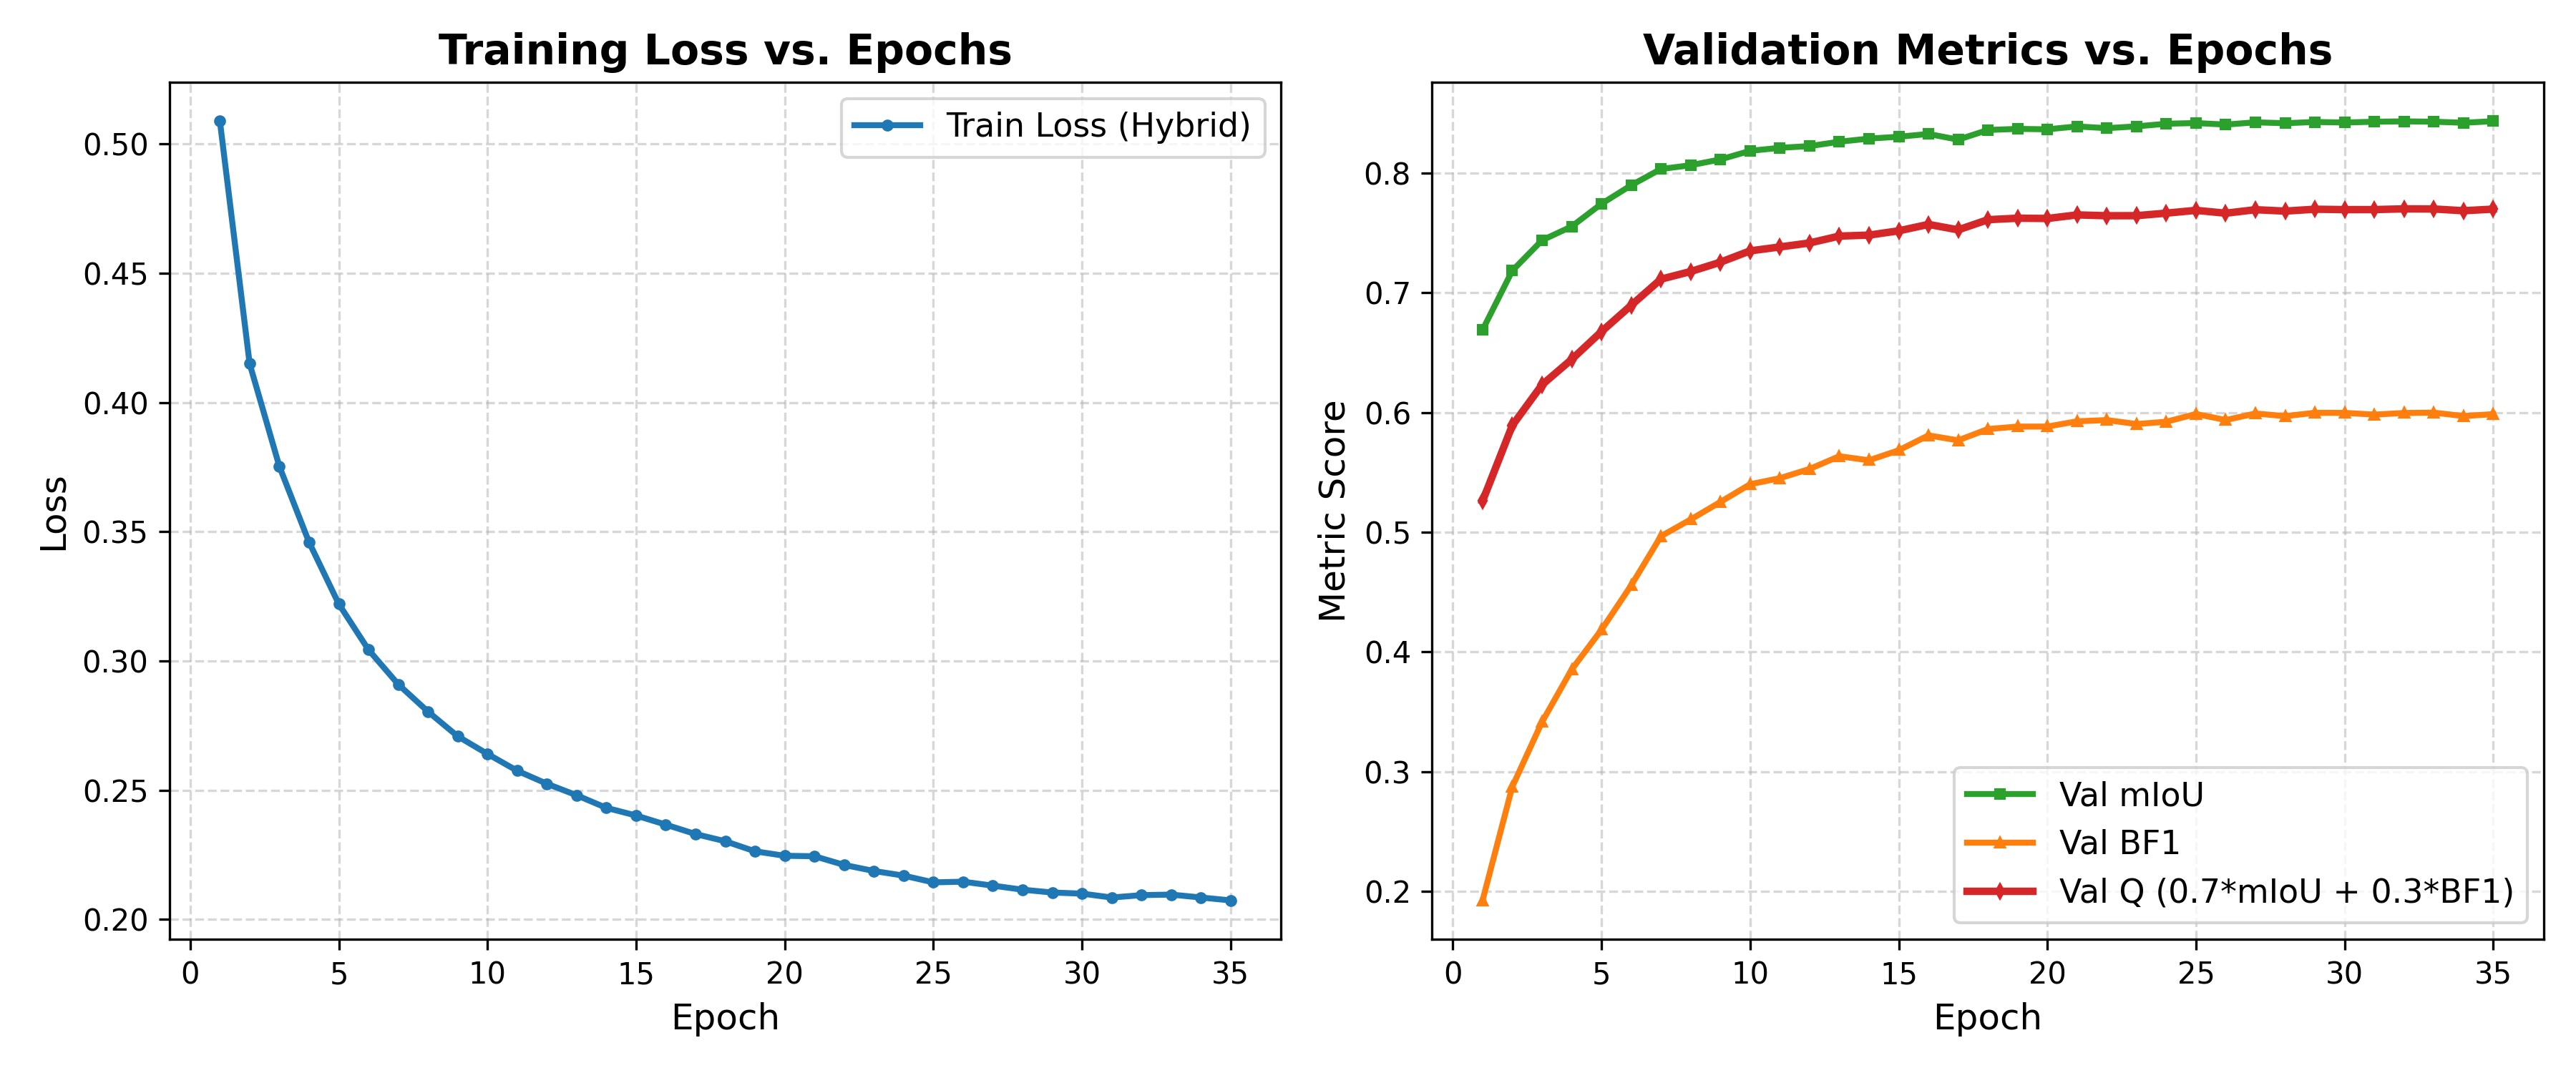
\includegraphics[width=0.88\linewidth]{training_curves_v3.png}
\caption{FastSegUNet training progress over 35 epochs on DUTS-TR. Left: hybrid training loss (0.5\,$\mathcal{L}_{\mathrm{BCE,edge}} + 0.5\,\mathcal{L}_{\mathrm{Dice}}$). Right: validation metrics (mIoU, Boundary F1, and $Q$) on the 1,055-image validation split.}
\label{fig:training-curves}
\end{figure}

Images are resized to $256\times256$ using \code{cv2.INTER\_AREA}; masks are resized using \code{cv2.INTER\_NEAREST} and thresholded at 128. The training pipeline applies horizontal flips, occasional vertical flips, and random brightness/contrast changes. The model receives RGB image tensors in the range $[0,255]$ and performs division by 255 in its forward pass.

The CPU used for the reported inference benchmark is an \textbf{AMD Ryzen 5 7520U with Radeon Graphics}. Inference is run on a single CPU thread.

\section{Quantitative Results}

The metrics below are taken from the final V3 evaluation record. mIoU is computed from the accumulated confusion matrix over a dataset, averaging the IoU for the foreground and background classes. Boundary F1 is computed per image using the assignment's $5\times5$ boundary matching tolerance, then averaged across the dataset.

\begin{table}[H]
\centering
\small
\caption{Segmentation quality on the validation, official test and captured-photo sets. Official cost metrics and CES are reported for DUTS-TE, as defined by the assignment.}
\resizebox{\linewidth}{!}{%
\begin{tabular}{@{}l r r r r r r r@{}}
\toprule
\textbf{Dataset} & \textbf{Images} & \textbf{mIoU} & \textbf{BF1} & \textbf{$Q$} & \textbf{$T_{\mathrm{CPU}}$} & \textbf{$S_{\mathrm{disk}}$} & \textbf{CES}\\
\midrule
Validation (DUTS-TR) & 1,055 & 0.8433 & 0.5995 & 0.7702 & -- & -- & --\\
\textbf{DUTS-TE (official)} & \textbf{5,019} & \textbf{0.6883} & \textbf{0.4298} & \textbf{0.6107} & \textbf{26.04 ms} & \textbf{148,255 B} & \textbf{0.5450}\\
Captured photos & 6 & 0.8164 & 0.5198 & 0.7274 & -- & -- & --\\
\bottomrule
\end{tabular}}
\end{table}

For DUTS-TE, the saved parameter file is 148,255 bytes (approximately 144.8 KiB). The timing is below the 50 ms budget. The score components are:
\[
\begin{aligned}
Q &= 0.70(0.6883)+0.30(0.4298) \approx 0.6107,\\
P_{\mathrm{time}} &= 0.20\left(\frac{26.0417}{50}\right) \approx 0.1042,\\
P_{\mathrm{size}} &= 0.10\left(\frac{148255}{4194304}\right) \approx 0.0035,\\
\mathrm{CES} &= 0.6107(1-0.1042-0.0035) \approx \mathbf{0.5450}.
\end{aligned}
\]
The measured mean CPU time is approximately 48\% below the 50 ms limit. The checkpoint occupies approximately 3.5\% of the 4 MiB reference size.

\clearpage
\section{Qualitative Results on Captured Photos}

The captured-photo set contains six images: \code{photo1}, \code{photo2}, \code{photo5}, \code{photo6}, \code{photo7} and \code{photo8}. Each image is evaluated against its manually prepared binary mask at $256\times256$. Figure~\ref{fig:captured-overlays} shows the manually annotated ground truth and V3 prediction as semi-transparent overlays. Green denotes ground truth and red denotes the V3 prediction.

\begin{figure}[H]
\centering
\begin{minipage}[t]{0.475\linewidth}
  \centering
  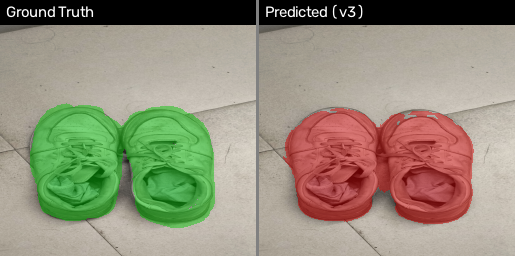
\includegraphics[width=0.94\linewidth]{captured/overlays/photo1_overlay.png}\\[1pt]
  {\footnotesize (a) \textbf{photo1}: Shoes (mIoU 0.931, BF1 0.549, $Q$ 0.817)}
\end{minipage}\hfill
\begin{minipage}[t]{0.475\linewidth}
  \centering
  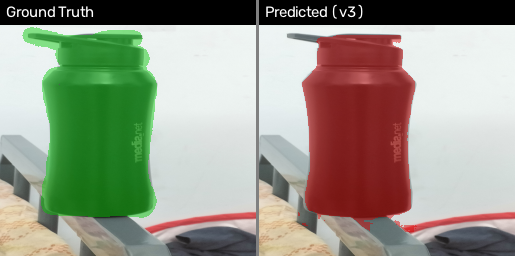
\includegraphics[width=0.94\linewidth]{captured/overlays/photo2_overlay.png}\\[1pt]
  {\footnotesize (b) \textbf{photo2}: Shaker bottle (mIoU 0.924, BF1 0.513, $Q$ 0.800)}
\end{minipage}\\[2pt]
\begin{minipage}[t]{0.475\linewidth}
  \centering
  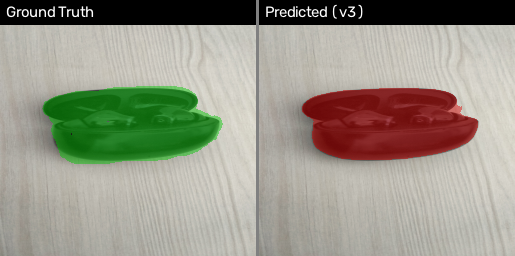
\includegraphics[width=0.94\linewidth]{captured/overlays/photo5_overlay.png}\\[1pt]
  {\footnotesize (c) \textbf{photo5}: Earbuds case (mIoU 0.948, BF1 0.672, $Q$ 0.865)}
\end{minipage}\hfill
\begin{minipage}[t]{0.475\linewidth}
  \centering
  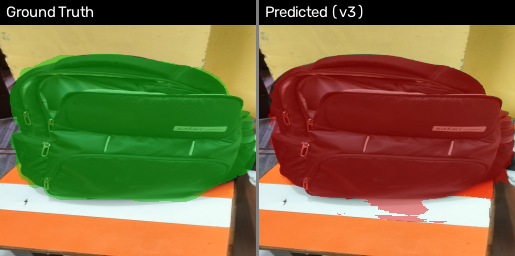
\includegraphics[width=0.94\linewidth]{captured/overlays/photo6_overlay.png}\\[1pt]
  {\footnotesize (d) \textbf{photo6}: Backpack (mIoU 0.928, BF1 0.600, $Q$ 0.830)}
\end{minipage}\\[2pt]
\begin{minipage}[t]{0.475\linewidth}
  \centering
  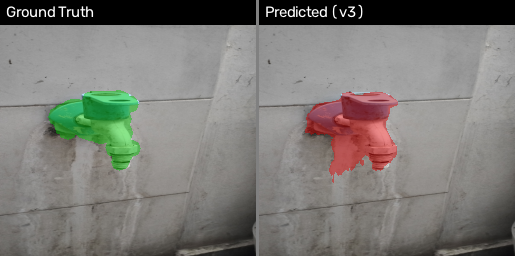
\includegraphics[width=0.94\linewidth]{captured/overlays/photo7_overlay.png}\\[1pt]
  {\footnotesize (e) \textbf{photo7}: Water tap (mIoU 0.855, BF1 0.635, $Q$ 0.789)}
\end{minipage}\hfill
\begin{minipage}[t]{0.475\linewidth}
  \centering
  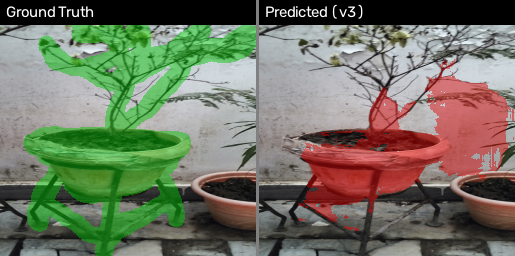
\includegraphics[width=0.94\linewidth]{captured/overlays/photo8_overlay.png}\\[1pt]
  {\footnotesize (f) \textbf{photo8}: Potted plant (mIoU 0.442, BF1 0.150, $Q$ 0.355)}
\end{minipage}\\[-4pt]
\caption{Captured-photo segmentation overlays. Green: ground-truth mask. Red: FastSegUNet (V3) prediction. In each panel, ground truth and prediction are displayed side by side.}
\label{fig:captured-overlays}
\end{figure}

The overlays show close agreement for the main object in photos 1, 2, 5 and 6. Photo 7 illustrates excess predicted foreground below the tap, while photo 8 shows a substantial omission of thin branches and parts of the plant support. These examples are discussed further in Section~\ref{sec:failure-analysis}.

\textbf{Scene-condition coverage.} The photographs visibly demonstrate at least three of the assignment's requested conditions:

\begin{table}[H]
\vspace{-3pt}
\centering
\small
\caption{Visible scene conditions represented by the captured-photo set.}
\begin{tabularx}{\linewidth}{@{}l X@{}}
\toprule
\textbf{Condition} & \textbf{Photographic evidence}\\
\midrule
Indoor and outdoor scenes & Indoor examples include the shoes (photo 1), earbuds case (photo 5) and backpack (photo 6). The potted plant (photo 8) is photographed outdoors.\\
Near and farther framing & The bottle (photo 2) and backpack (photo 6) are framed closely, while the tap (photo 7) occupies a much smaller part of a wider wall view.\\
Cluttered background & Photo 8 includes multiple pots, the plant stand, branches and a textured outdoor setting around the main object.\\
\bottomrule
\end{tabularx}
\vspace{-3pt}
\end{table}

The photographs do not provide sufficiently clear visual evidence to claim a specific tube-light setup or a deliberate partial-occlusion case, so those conditions are not counted toward the coverage statement.

\clearpage
\section{Discussion}

\subsection{V2-to-V3 experiment}

V3 changed two architectural choices relative to V2: the channel width was reduced from \code{base\_ch = 24} to 16, while the refinement block was moved back to full $256\times256$ resolution. The resulting DUTS-TE measurements are:

\begin{table}[H]
\centering
\small
\caption{V2 and V3 DUTS-TE comparison.}
\begin{tabular}{@{}l r r r@{}}
\toprule
\textbf{Metric} & \textbf{V2} & \textbf{V3} & \textbf{Change}\\
\midrule
mIoU & 0.6980 & 0.6883 & $-0.0097$\\
Boundary F1 & 0.4559 & 0.4298 & $-0.0261$\\
$Q$ & 0.6253 & 0.6107 & $-0.0146$\\
$T_{\mathrm{CPU}}$ & 42.504 ms & 26.042 ms & $-38.7\%$\\
$S_{\mathrm{disk}}$ & 249,631 B & 148,255 B & $-40.6\%$\\
CES & 0.5153 & \textbf{0.5450} & $+0.0297$\\
\bottomrule
\end{tabular}
\end{table}

Although V3 has lower mIoU, BF1 and $Q$ than V2, its lower inference time and smaller checkpoint reduce the cost penalties sufficiently to improve CES from 0.5153 to 0.5450. The intended improvement in boundary quality was not observed on DUTS-TE.

The comparison changes both channel width and refinement resolution at the same time, so it does not isolate the effect of either choice. A plausible explanation is that reducing channel width lowered representational capacity enough to offset any benefit from full-resolution refinement. The result therefore demonstrates a measured quality--efficiency trade-off, rather than proving that one architectural factor is more important in general.

\subsection{Validation-to-test performance gap}

The validation $Q$ of 0.7702 is higher than the DUTS-TE $Q$ of 0.6107. The same difference is visible in both mIoU and BF1. This indicates that the model performs less strongly on the held-out test set than on the validation split. Differences in sample difficulty, image characteristics or the limited capacity of the compact network are possible explanations; the reported metrics alone do not establish a single cause.

\clearpage
\section{Failure Analysis}\label{sec:failure-analysis}

\subsection{Photo 8: substantial under-segmentation}

Photo 8 is the weakest captured example, with mIoU 0.4423, BF1 0.1500 and $Q$ 0.3546. Its ground-truth foreground contains 25,507 pixels, while the model predicts 15,089 foreground pixels. The predicted foreground area is therefore approximately 59.2\% of the ground-truth area.

The overlay confirms that the prediction retains much of the pot and central trunk but misses a substantial part of the thin upper branches and lower support structure. The branches occupy only a small number of pixels after resizing and repeated spatial downsampling, making them difficult to preserve. The surrounding branches, neighbouring pot and textured outdoor setting also create a visually cluttered background. These are plausible contributing factors rather than experimentally isolated causes.

\subsection{Photo 7: over-segmentation}

Photo 7 has mIoU 0.8553, BF1 0.6346 and $Q$ 0.7891. The predicted foreground contains 5,152 pixels compared with 4,318 pixels in the ground truth, a net excess of 834 pixels (approximately 19.3\% of the ground-truth foreground area). This indicates an over-segmentation tendency in this example.

The overlay shows that the predicted foreground extends below the tap into a region of the surrounding wall. A nearby stain or shadow may share visual characteristics with the tap and contribute to this leakage, although the image alone cannot establish the model's internal reason for the error. The area difference is a net difference; it should not be interpreted as the exact number of false-positive pixels.

\section{Conclusion}

FastSegUNet obtains an official DUTS-TE CES score of \textbf{0.5450}, with mean CPU inference time of \textbf{26.04 ms per image} and a saved parameter file of \textbf{148,255 bytes}. It remains within the assignment's 50 ms timing budget and has a compact checkpoint. The DUTS-TE results also show that boundary quality remains a limitation, with BF1 lower than mIoU.

The V2-to-V3 comparison illustrates the trade-off between segmentation quality and inference cost: V3's quality score decreased, but the runtime and model-size reductions improved the final CES score. The captured-photo results show generally strong performance on five of the six examples, alongside a substantial under-segmentation failure on photo 8. The six captured-photo overlays and the visible scene-condition evidence provide a qualitative complement to the aggregate metrics.

\vspace{5pt}
\hrule
\vspace{3pt}
{\small\color{muted}\textit{End of report.}}

\end{document}